\documentclass[a4paper]{jpconf}
\usepackage{graphicx}
\begin{document}
\title{PyFAI, a versatile library for azimuthal regrouping}

\author{J\'er\^ome Kieffer, Dimitrios Karkoulis}

\address{European Synchrotron Radiation Facility; 6 rue Jules Horowitz;
38043 Grenoble; France}

\ead{jerome.kieffer@esrf.fr}

\begin{abstract}
$2D$ area detectors like \textsc{ccd} or pixel detectors have become popular
in the last 15 years for diffraction experiments (e.g. for \textsc{waxs},
\textsc{saxs}, single crystal and powder diffraction (\textsc{xrpd})).
These detectors have a large sensitive area of millions of pixels with  high
spatial resolution. The software package pyFAI has been designed to reduce
\textsc{saxs}, \textsc{waxs} and \textsc{xrpd} images taken with those detectors
into $1D$ curves (azimuthal integration) usable by other software for
in-depth analysis such as Rietveld refinement, or $2D$ images (a radial
transformation named \textit{caking}).
As a library, the aim of pyFAI is to be integrated into other tools like
PyMca or \textsc{edna} with a clean pythonic interface.
However pyFAI features also command line tools for batch processing, converting
data into {\em q-space} (q being the momentum transfert) or 2$\theta$-space
($\theta$ being the Bragg angle) and a calibration graphical interface for
optimizing the geometry of the experiment using the Debye-Scherrer rings of a
reference sample.  
PyFAI shares the geometry definition of \textsc{spd} but can directly import
geometries determined by the software \textsc{fit2d}.
PyFAI has been designed to work with any kind of detector and geometry
(transmission or reflection) and relies on FabIO, a library able to read more 
than 20 image formats produced by detectors from 12 different manufacturers.
During the transformation from cartesian space $(x,y)$ to polar
space $(2\theta, \chi )$, both local and total intensities are conserved
in order to obtain accurate quantitative results. Technical details on how this
integration is implemented and how it has been ported to native code and
parallelized on graphic cards are discussed in this paper.
\end{abstract}

\section{Introduction}

With the advent of hyperspectral experiments like diffraction tomography in the
world of synchrotron radiation, existing software tools for azimuthal
integration like \textsc{fit2d}\cite{fit2d1996} and \textsc{spd}\cite{spd} reached their
performance limits owing to the fast data rate needed by such experiments. Even
when integrated into massively parallel frameworks like
\textsc{edna}\cite{edna}, such stand-alone programs, due to their monolithic
nature, cannot keep the pace with the data flow of new detectors.
Therefore we decided to implemente from scratch a novel azimuthal integration
tool which is designed to take advantage of modern parallel hardware features
(if available).

\section{Python Fast Azimuthal Integration}
PyFAI is implemented in Python programming language, which is open
source and already very popular for scientific data analysis (PyMca\cite{pymca},
PyNX\cite{pynx}, \ldots). 

\subsection{Geometry and calibration}
PyFAI and \textsc{spd}\cite{spd} share the same 6-parameter geometry definition:
distance, point of normal incidence (2 coordinates) and 3 rotations around
the main axis; these parameters are saved in text files usually with the
\textit{.poni} extension. The program \textit{pyFAI-calib} helps calibrating the
experimental setup using a constrained least squares optimization on the
Debye-Scherrer rings of a reference sample ($LaB_6$, silver
behenate, \ldots). Alternatively, geometries calibrated using 
\textsc{fit2d}\cite{fit2d1996} can be imported into pyFAI; including geometric
distortions (i.e. optical-fiber tapers distortion) and described as
\textit{spline-files}.

\subsection{PyFAI executables}
PyFAI was designed to be used by scientists needing a simple and effective tool
for azimuthal integration. Two command line programs \textit{pyFAI-waxs} and
\textit{pyFAI-saxs} are provided with pyFAI for performing the
integration of one or more images. The \textsc{waxs} version outputs results in
$2\theta /I$,  whereas the \textsc{saxs} version outputs $q/I(/\sigma )$.
Options for these programs are parameter file (\textit{poni-file}) describing
the geometry and the mask file. They can also do some pre-processing like
dark-noise subtraction and flat-field correction (solid-angle correction is done by
default).

\subsection{Python library}
PyFAI is first and foremost a library: a tool of the scientific
toolbox built around IPython\cite{ipython} and NumPy\cite{numpy} to
perform data analysis either interactively or via scripts.
Figure \ref{notebook} shows an interactive session where an integrator is
created, and an image loaded and integrated before being plotted.

\begin{figure}[h]
\begin{center}
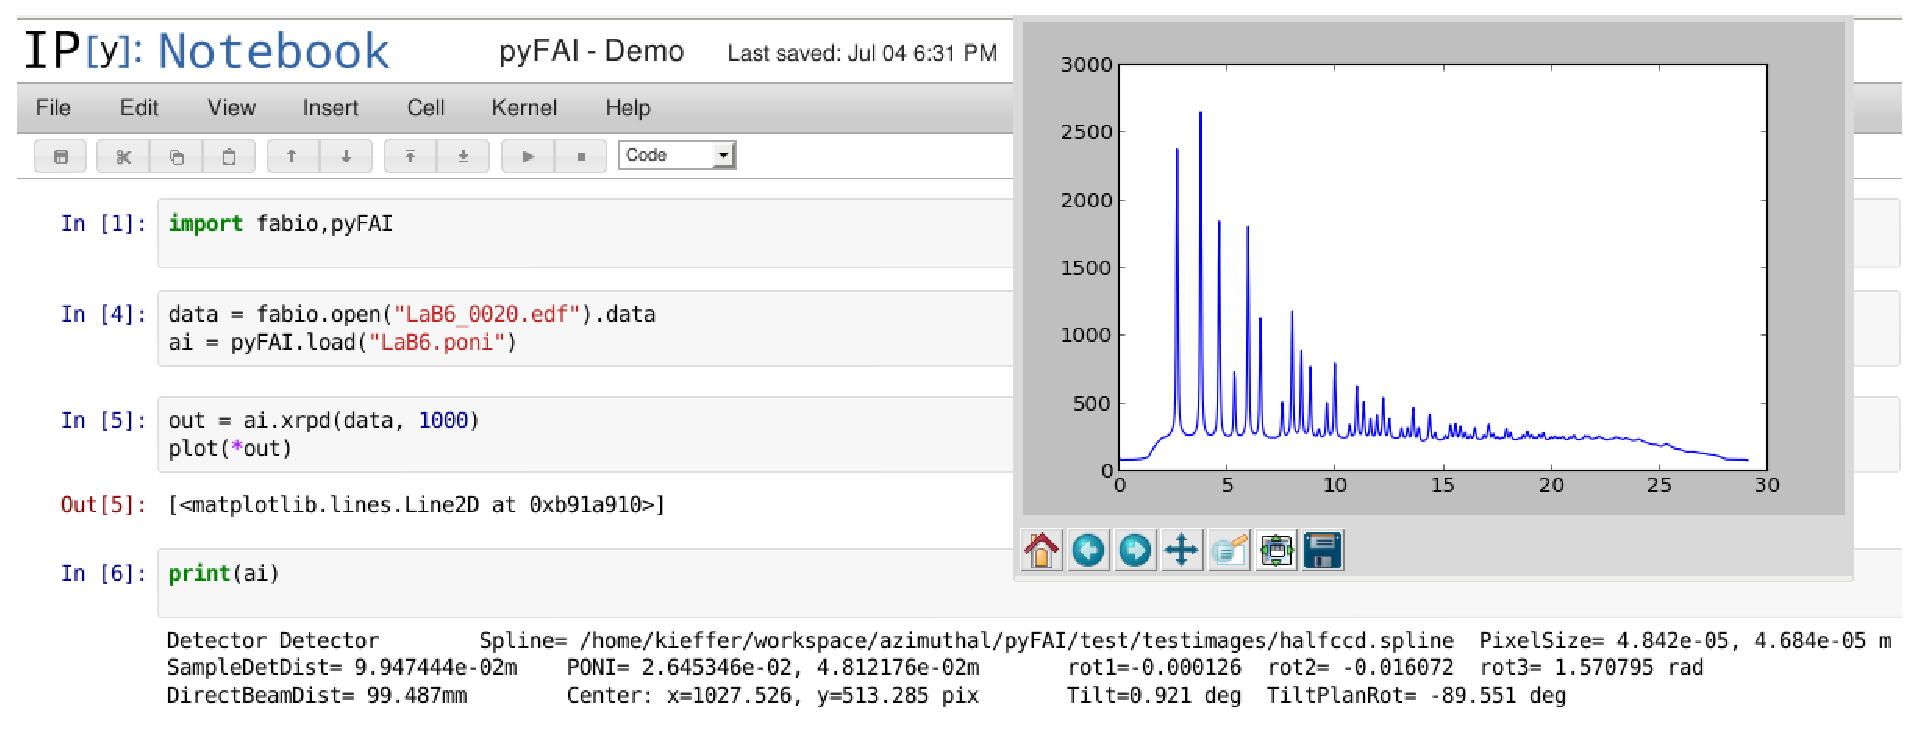
\includegraphics[width=15cm]{img/notebook-l.eps}
\caption{\label{notebook} Example of interactive use of FabIO and pyFAI in the
notebook edition of IPython.}
\end{center}
\end{figure}

\section{Regrouping mechanism}
In pyFAI, regrouping is performed using a histogram like algorithm.
Each pixel of the image is associated to its polar coordinates
$(2\theta , \chi )$ or $(q, \chi )$, then a pair of histograms versus
$2\theta$ (or $q$) are built, one non weighted for measuring the number of
pixels falling in each bin and another weighted by pixel intensities (after
dark-current subtraction, and corrections for flat-field,
solid-angle and polarization).
The division of the weighted histogram by the number of pixels per bin gives
the diffraction pattern.
$2D$ regrouping (called \textit{caking} in \textsc{fit2d}) is obtained in the
same way using two-dimensional histograms over radial ($2\theta$ or $q$) and azimuthal angles
($\chi$).

\subsection{Pixel splitting algorithm}
Powder diffraction patterns obtained by histogramming have a major weakness where
pixel statistics are low.
%: a high level of noise is observed close to the beam-stop.
A manifestation of this weakness becomes apparent in the $2D$-regrouping where
most of the bins close to the beam-stop are not populated by any pixel.
In Figure \ref{rough}, many pixels are missing in the low $2\theta$ region, due
to the arbitrary discretization of the space in pixels as intensities were
assigned to each pixel center which does not reflect the physical reality of the
scattering experiment.
% PyFAI considers an homogeneous distribution :
% photons arrived to any point of the pixel. Hence we ons (not even considering the point
% spread function).
% In Figure \ref{smooth}, the pixel splitting algorithm removes those artifacts.
PyFAI solves this problem by pixel splitting (Figure \ref{smooth}): in 
addition to the pixel position, its spatial extension is calculated and each
pixel is then split and distributed over the corresponding bins, the intensity
being considered as homogeneous within a pixel and spread accordingly. 

\begin{figure}[h]
\begin{minipage}{8cm}
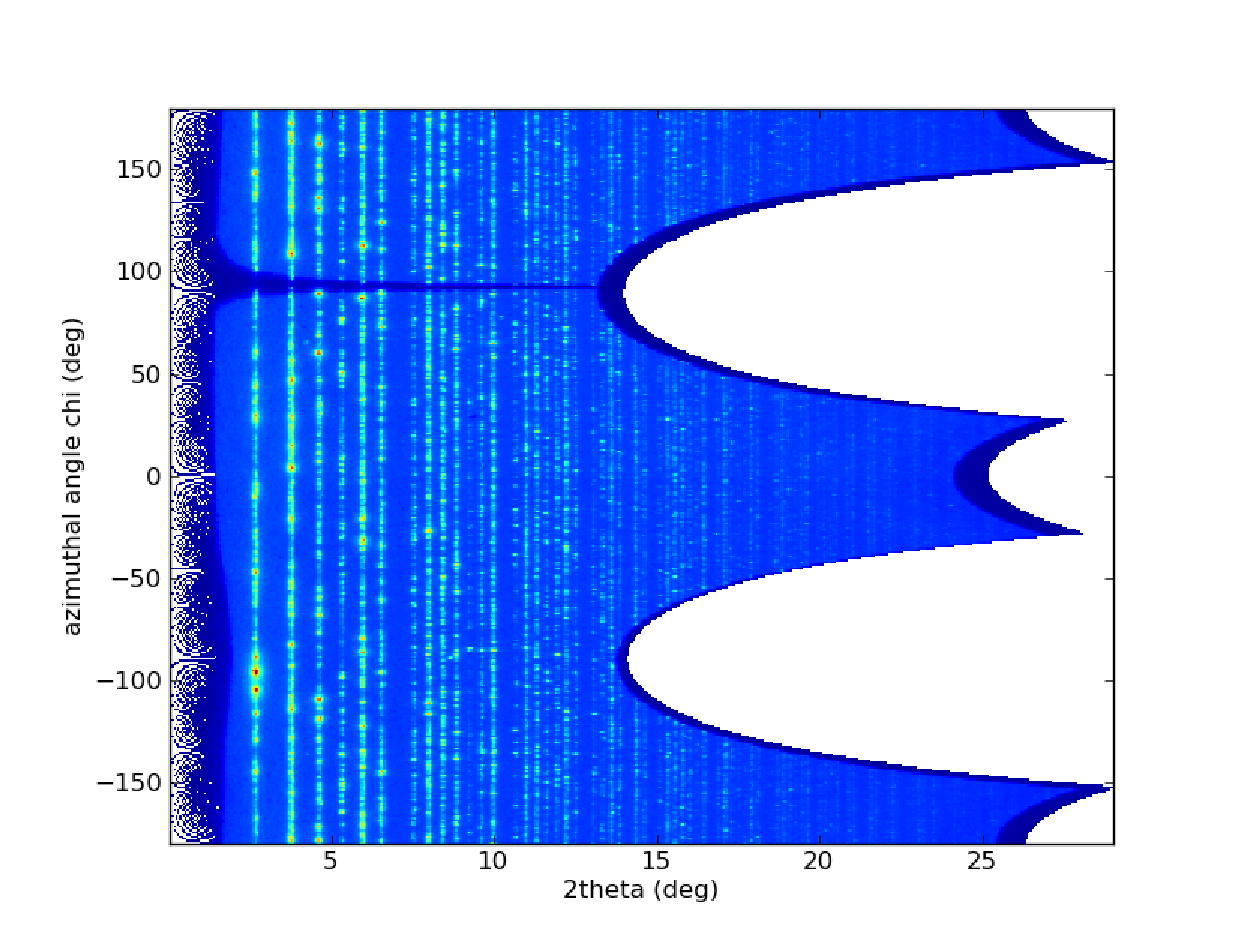
\includegraphics[width=8cm]{img/2Dhistogram.eps}
\caption{\label{rough}$2D$-regrouped image without pixel splitting. Note
the missing pixels near the beam stop and the high-frequency noise patterns.}
\end{minipage}\hspace{5mm}
\begin{minipage}{8cm}
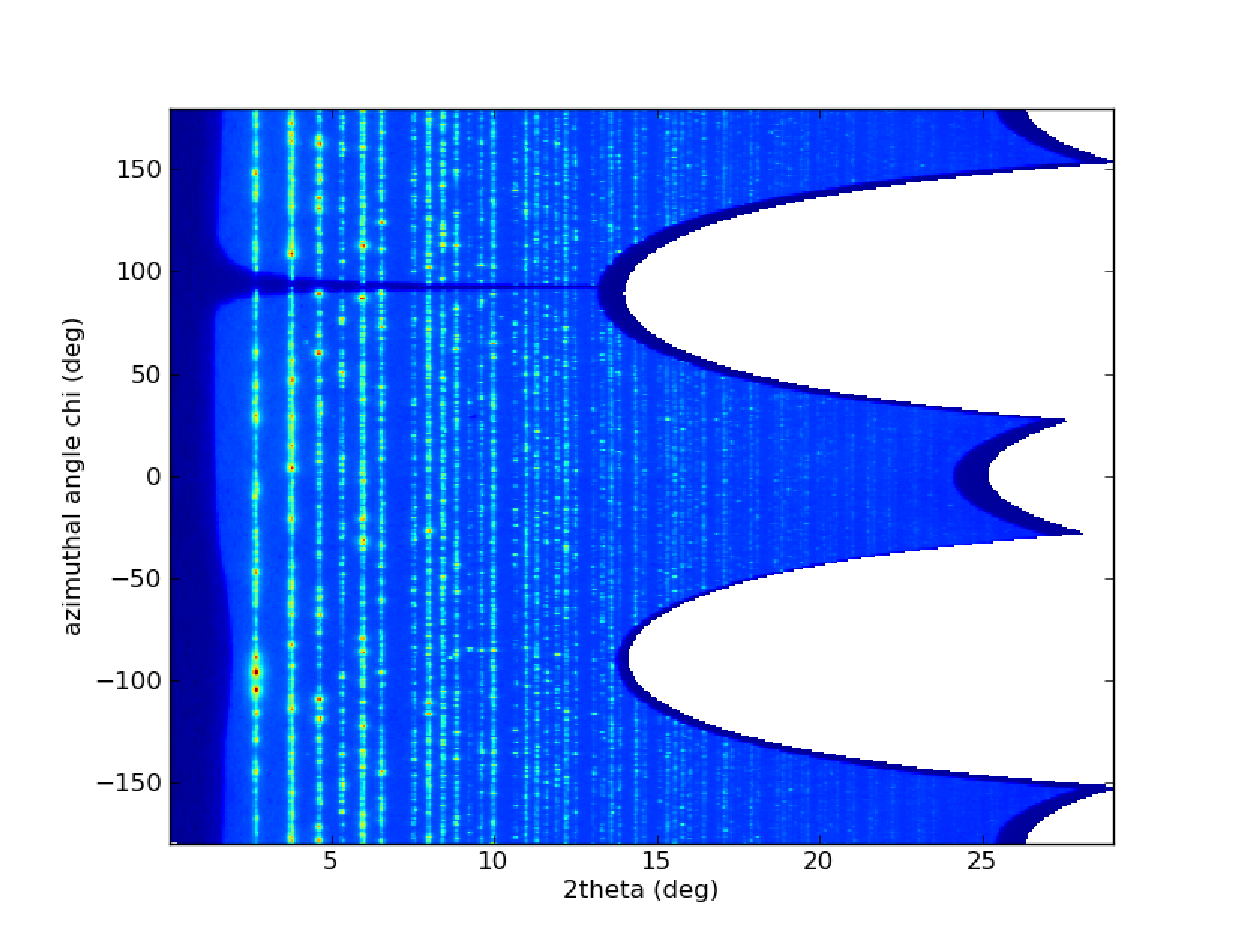
\includegraphics[width=8cm]{img/2DwithSplit.eps}
\caption{\label{smooth}$2D$-regrouped image with pixel splitting. The
transformation of a smooth image remains smooth.}
\end{minipage}
\end{figure}


\subsection{Performances and migration to native code}
Originally, regrouping was implemented using the histogram provided by
NumPy\cite{numpy}, then re-implemented in Cython\cite{cython} with pixel
splitting to achieve a four-fold speed-up.
The computation time scales like O(N) with the size of the input image.
The number of output bins shows only little influence; overall the single
threaded Cython implementation has been stated at 30 Mpix/s (on a 3.4 GHz Intel
core i7-2600).

\subsection{Graphic card implementation}
Graphics Processing Units (\textsc{gpu}s) are composed of hundreds of
arithmetic logic units; they are optimized for highly
parallel algorithms with speed-up factors reaching up to 3 orders of magnitude
over sequential codes running on Central Processing Units (\textsc{cpu}).
While histograms do not fall into this category, they can nevertheless be
ported to a \textsc{gpu} architecture efficiently.
In order to benefit from \textsc{gpu} acceleration,
the Open Computing Language\cite{opencl} (OpenCL) was used. OpenCL can make use
of multiple different devices such as \textsc{cpu}s and \textsc{gpu}s with very
different features and capabilities.
OpenCL allows the code to work on multiple \textsc{cpu} cores, which is 
useful for validation purposes.
As azimuthal integration is a reduction
of millions of pixels into hundreds of bins, double-precision arithmetic is
preferred, which however is not available on all OpenCL devices.
Table \ref{perfs} summarizes the execution times for images recorded on 
various detectors on a dual-processor computer, either using 
1) single threaded implementation in Cython,
2) OpenCL on 12 \textsc{cpu}-cores,
3) OpenCL on a nVidia Tesla C2075 (448 \textsc{gpu}-cores),
4) OpenCL on a nVidia GTX580 (512 \textsc{gpu}-cores) and
5) OpenCL on an AMD FirePro v7800 (1440 \textsc{gpu}-cores but only in single
precision).

\begin{table}[h]
\caption{\label{perfs}Execution time in milliseconds measured on a
Dell T7500 with two Intel Xeon X5690 @3.47GHz and various \textsc{gpu}s.}
%: C2075 and GTX580 are professional
%and consumer grade Fermi class nVidia \textsc{gpu} with 512 cores.\\
% The table reports execution time measured in milliseconds for various
% detectors in double precision (except for the AMD FirePro v7800: single precision).}
\vspace{1mm}
\begin{center}
\begin{tabular}{|l|c||c|c||c|c|c|c|}
\hline
Detector type   & Image size 	& \multicolumn{2}{|c||}{\textsc{cpu} X5690}& \multicolumn{4}{|c|}{OpenCL $1D$ regrouping} \\
					& in Mpix		& $1D$	&	$2D$	&	X5690	&	C2075	&	GTX580	&	FirePro* \\
\hline
Pilatus-1M 			& 1  			& 34.4  &	63.1	&	13.9	&	7.2		&	6.3		&	13.8 \\
Half-Frelon 		& 2  			& 76.6  &   132.4   &	23.4	&	14.4	&	12.2	&	18.8 \\
Frelon 				& 4  			& 165.0	&	269.4   &	52.6	&	34.1	&	28.2	&	40.0 \\
Pilatus-6M 			& 6  			& 232.0	&	350.7	&	74.4	&	49.8	&	40.7	&	48.1 \\
Fairchild 			& 16 			& 613.9	&	849.7   &	158.9	&	99.0	&	96.4	&	95.6 \\
\hline
\end{tabular}
\end{center}
\end{table}

The OpenCL implementation of pyFAI is very fast on \textsc{gpu} providing an
extra five-fold speed-up over the \textsc{cpu} implementation. The
profiling of the code revealed new bottlenecks which will be addressed in future
optimizations. The OpenCL implementation of the $2D$ regrouping will also be
finalized in a future release.

\section{Conclusion}
The library pyFAI was developed with two main goals:
\begin{itemize}
\item Performing azimuthal integration with a clean programming interface.
\item No compromise on the quality of the results is accepted: a careful
management of the geometry and precise pixel splitting ensures total and
local intensity preservation.
\end{itemize}
PyFAI is the first implementation of an azimuthal integration algorithm on
a \textsc{gpu} as far as we are aware of, and the stated twenty-fold speed up
opens the door to a new kind of analysis, not even considered before:
a ten-line Python script is sufficient to reduce the data of a whole
diffraction-tomography experiment. Such analysis takes a few minutes using
pyFAI on a 60 x 200 frames dataset whereas it used to take days with existing
tools.
We believe PyFAI is able to sustain the data streams from the next generation
high-speed detectors.

\subsection*{Acknowledgments}
The authors would like to express their most sincere appreciation to their
colleagues and especially M. S\'anchez del R\'io for suggesting
the usage of weighted histograms; P. B\"osecke for the provision of the
experiment geometry setup; V. A. Sol\'e for his expertise on developing  native 
code under Windows and J. Wright for precise specifications and validations.
Porting pyFAI to \textsc{gpu} would have not been possible without the financial
support of LinkSCEEM-2 (RI-261600).

\subsection*{Appendix}
PyFAI is open-source software released under the GPL licence.
As of July 2012, pyFAI version 0.6, which includes OpenCL
acceleration, is available on the \textsc{epn} campus forge\cite{forge}.
PyFAI depends on Python v2.6 or v2.7, NumPy\cite{numpy} and OpenCL\cite{opencl}.
In order to be able to read images from various detectors, pyFAI relies on the
FabIO\cite{fabio} library available from SourceForge.  
In addition, the graphical user interface for calibration of diffraction setups
uses matplotlib\cite{matplotlib}, SciPy\cite{scipy}, and FFTw3\cite{fftw}.
C, C++ compilers and Cython\cite{cython} are needed to build pyFAI from
sources.
PyFAI is packaged and available in common Linux distributions like Debian
7.0 and Ubuntu 12.04. Installer packages for Windows are also
available on the \textsc{epn} campus forge.

\section*{References}
\bibliographystyle{iopart-num}
\bibliography{biblio}
\end{document}
